\chapter{A tervezett architektúra}

TODO: Gyors bevezető arról, hogy külön AWS accountba dolgoztam és felügyeltem a költségeim.

\section{Logikai felépítés}

TODO: High-level leírása az AWS accounton belüli/datacenteren belüli hálózati kommunikáció rétegeinek.

A rendszer egyszerűsített felülnézetét, az AWS-erőforrások összeköttetését jól összefoglalja az \refstruc{fig:architect}.

\begin{figure}[ht]
	\centering
	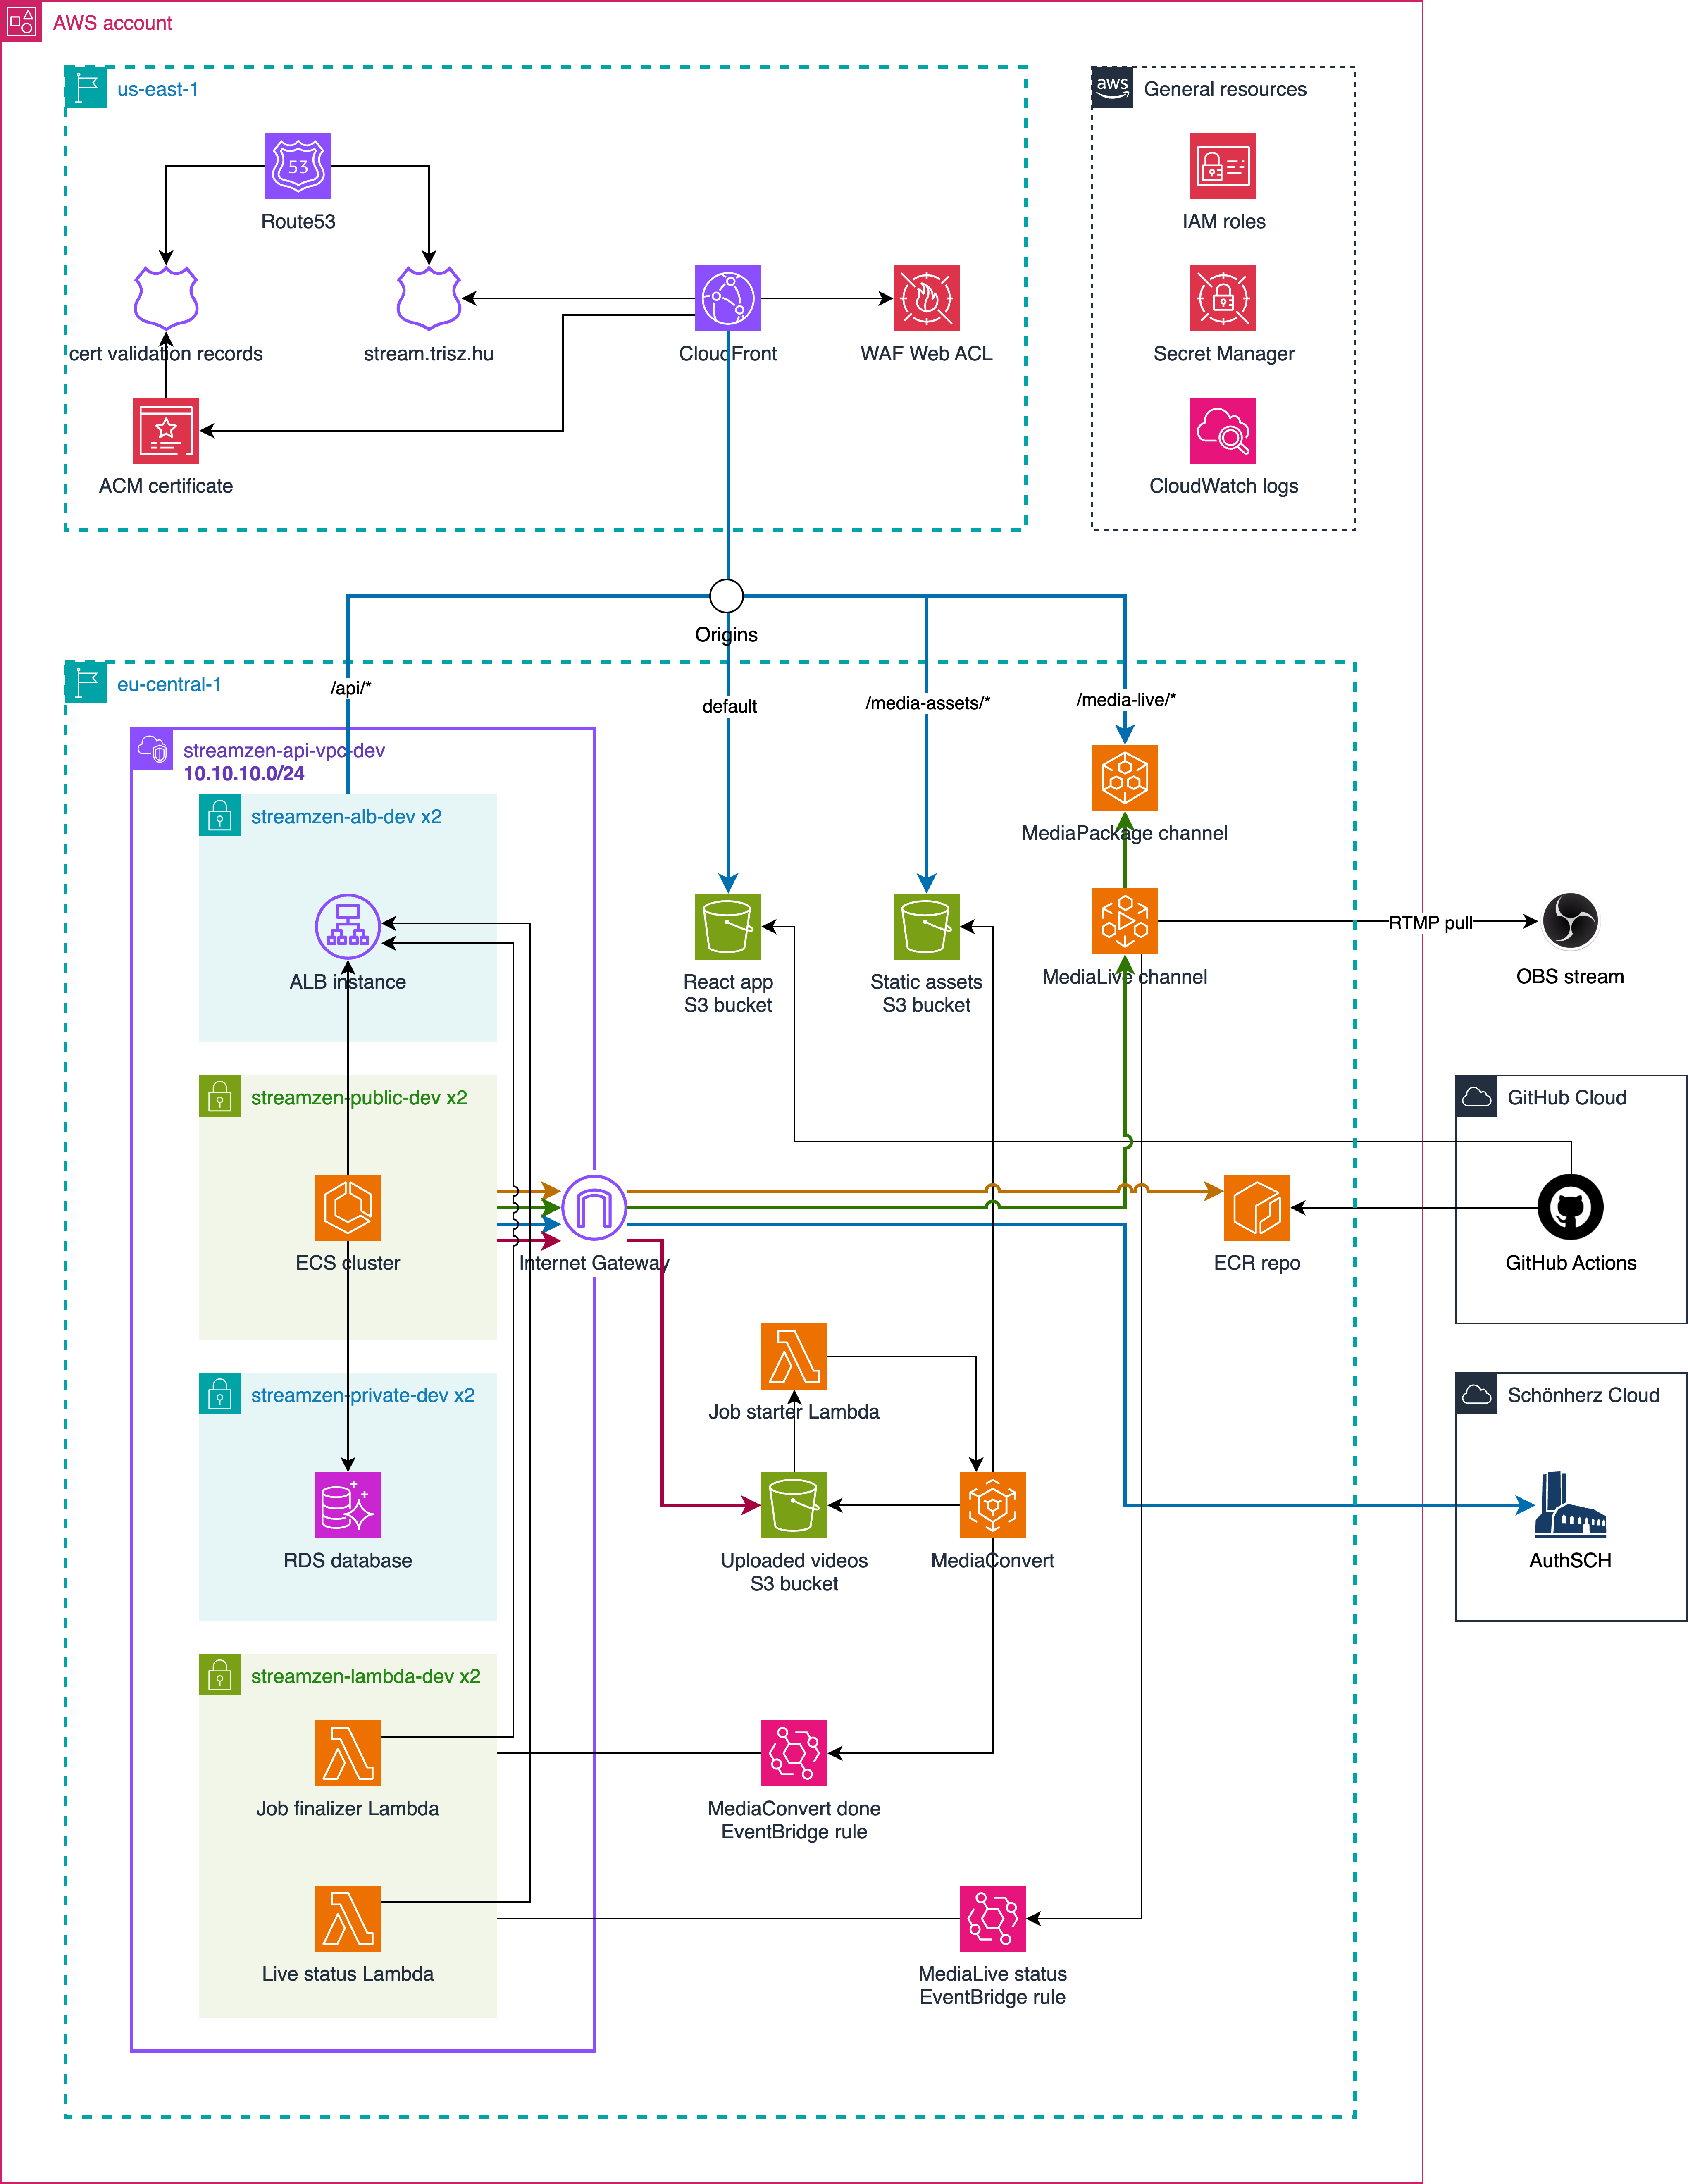
\includegraphics[width=155mm, keepaspectratio]{figures/dipterv_architect.png}
	\caption{Az AWS-fiók erőforrásainak logikai kapcsolata.}
	\label{fig:architect}
\end{figure}

\subsection{Összehasonlítás egy hasonló rendszerrel}

A tervek igazolásához segítségül kerestem az interneten nyílt forráskódú hasonló megoldásokat is. Megtaláltam a Technische Universität München (TUM) egy hallgatói csoportja, a TUM-Dev által fejlesztett az egyetemen is használt VoD és live streaming szolgáltatását, a GoCastot\footnote{\url{https://github.com/TUM-Dev/gocast}}. Ez a rendszer önállóan hosztolható szoftvereket komponál össze, nem felhőnatív. A rendszerben hasonló absztrakt terveket lehet megfigyelni az én megoldásaimhoz (\refstruc{fig:gocast}), ugyanígy HLS-sel szolgálják ki a tartalmakat (lásd \emph{TUM-Live Edge} példányok), viszont a live streamingre saját több portos workereket alkalmaznak (lásd \emph{TUM-Live-Worker} példányok), lehetőség ad viszont saját streamerből RTMP-n keresztül feltölteni élő közvetítést, ahogy én is megvalósítom a saját megoldásomban. Külön mikroszolgáltatás biztosítja a live és VOD streamingen kívüli funkcionalitásokat, a TUM-Live. Ez a megoldás nem teszi lehetővé, hogy a rendszeren kívül készült videót lehessen feltölteni és VOD-ként elérhetővé tenni rajta keresztül.

\begin{figure}[ht]
	\centering
	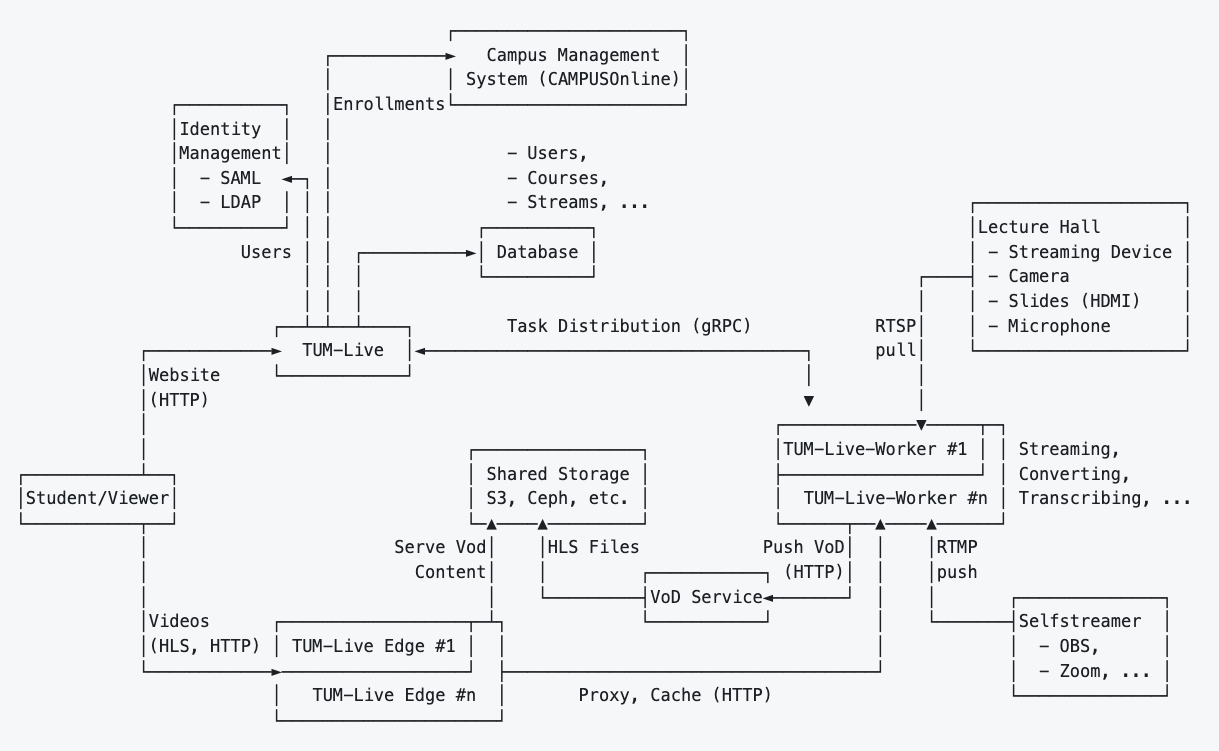
\includegraphics[width=140mm, keepaspectratio]{figures/gocast.png}
	\caption{A GoCast architektúrája a dokumentációból.}
	\label{fig:gocast}
\end{figure}

\section{Video-on-Demand kiszolgálás folyamata}

TODO: High-level leírása a VoD kiszolgálás folyamatának, megemlítve, melyik választott szolgáltatások vesznek részt ebben.

\begin{figure}[ht]
	\centering
	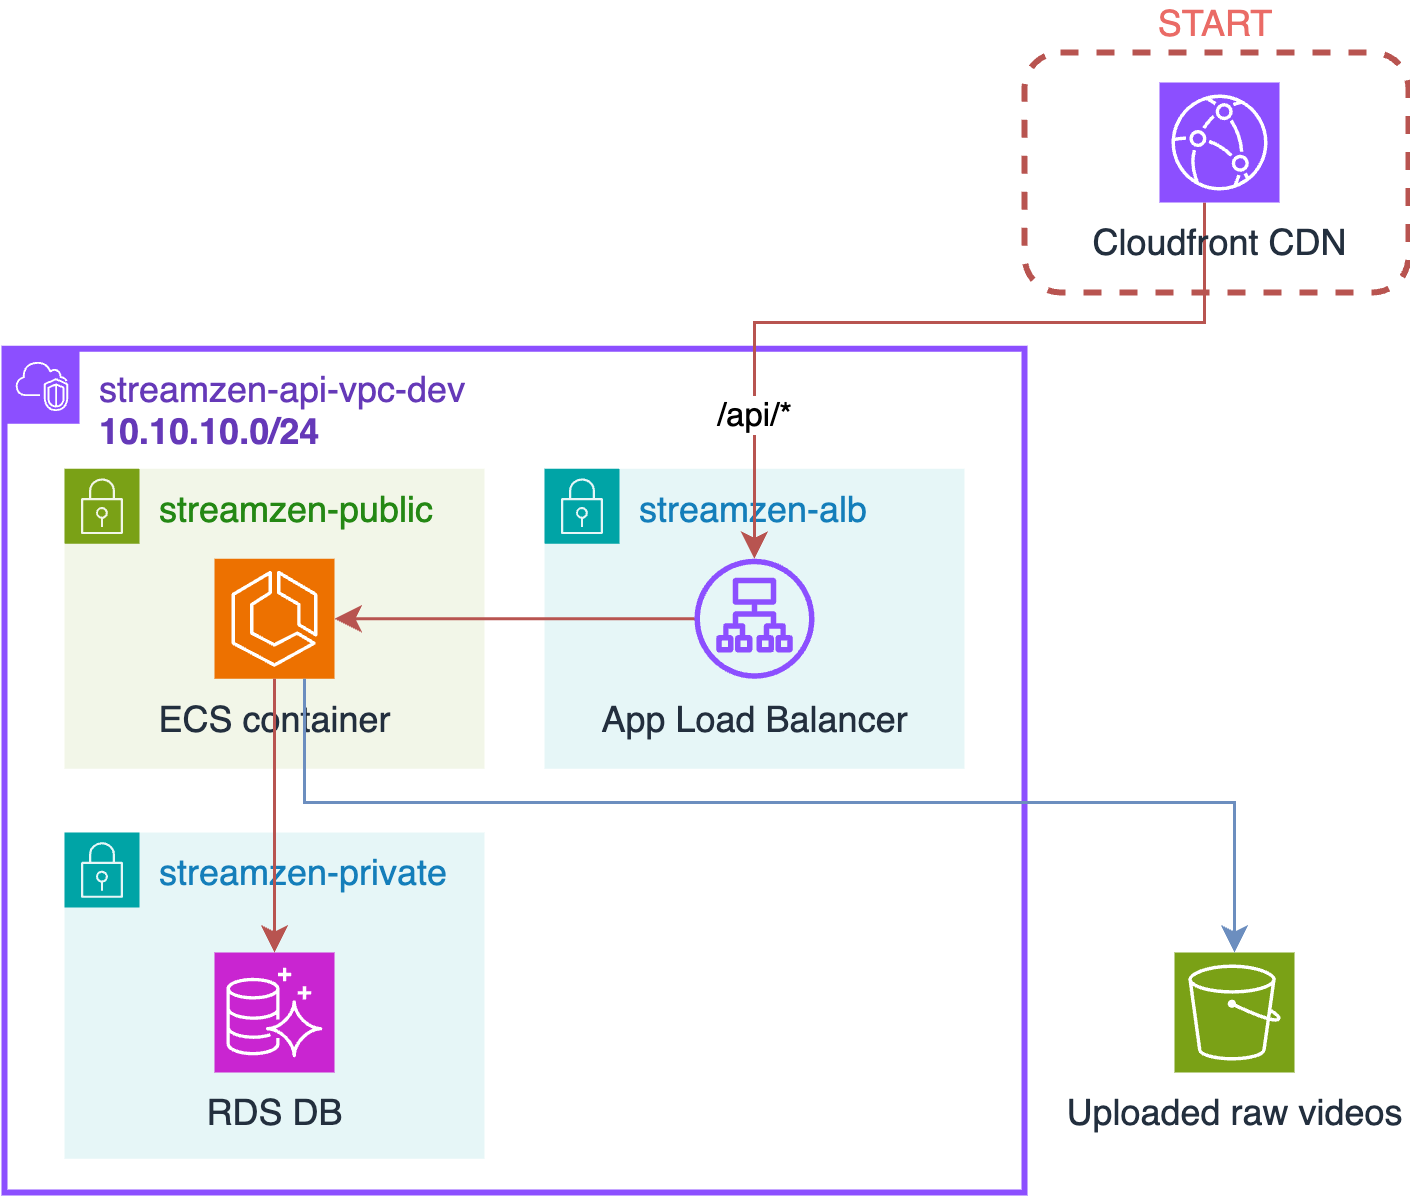
\includegraphics[width=120mm, keepaspectratio]{figures/dipterv_vod1.png}
	\caption{Folyamatábra a VOD tartalom feltöltéséről.}
	\label{fig:vod1}
\end{figure}

\begin{figure}[ht]
	\centering
	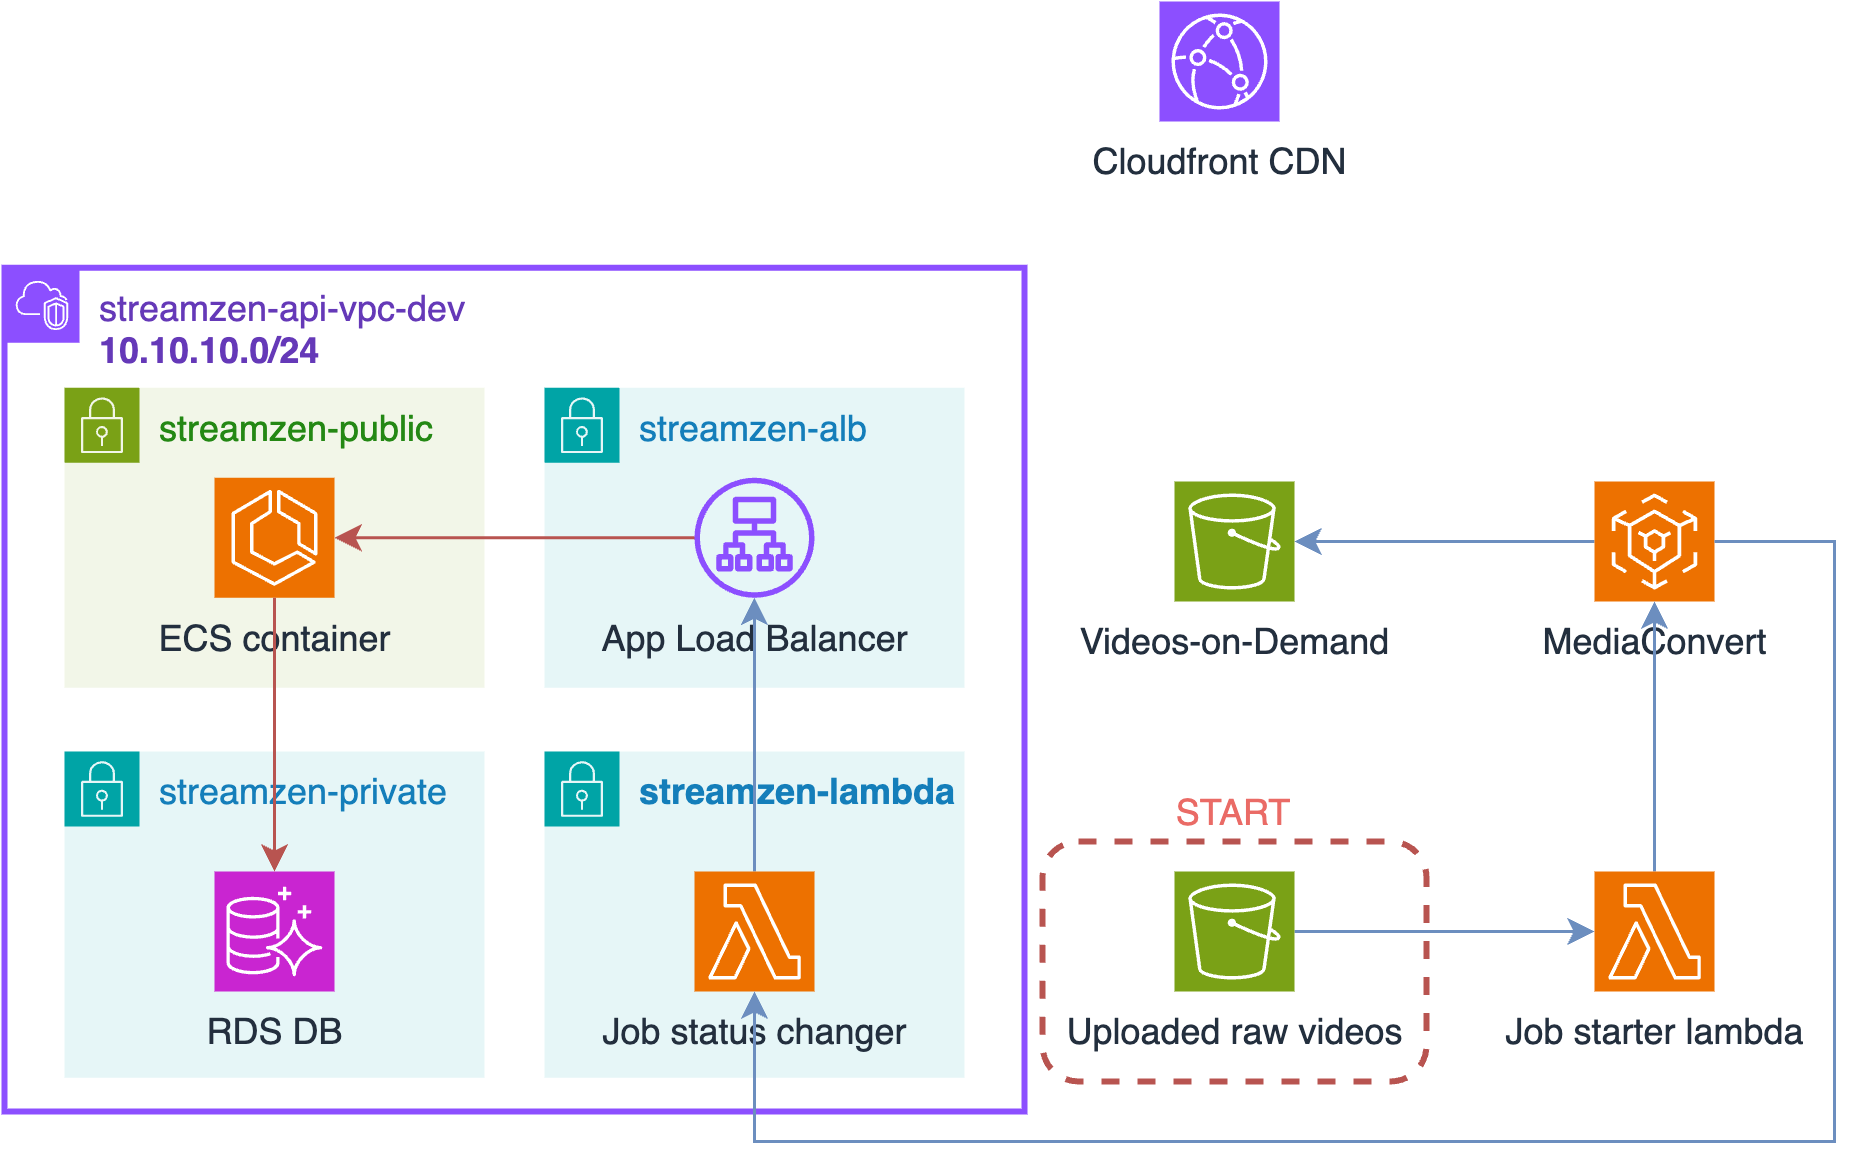
\includegraphics[width=120mm, keepaspectratio]{figures/dipterv_vod2.png}
	\caption{Folyamatábra a feltöltés utáni videófeldolgozásról.}
	\label{fig:vod2}
\end{figure}

\begin{figure}[ht]
	\centering
	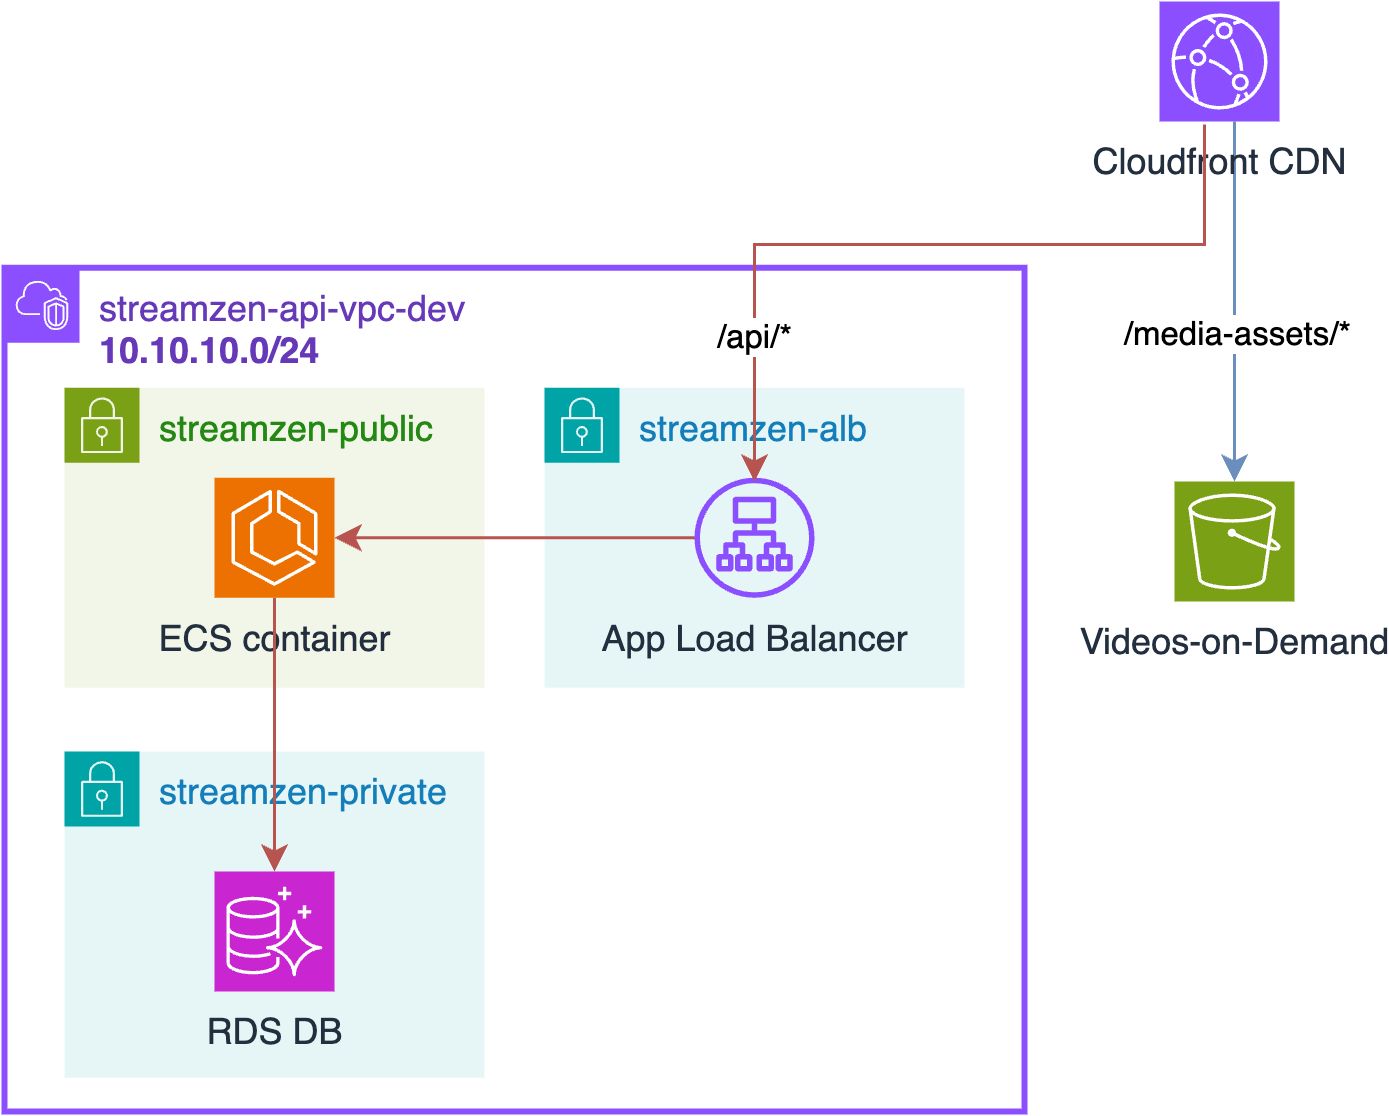
\includegraphics[width=120mm, keepaspectratio]{figures/dipterv_vod3.png}
	\caption{Folyamatábra a VOD tartalom lejátszásáról.}
	\label{fig:vod3}
\end{figure}

\section{Live streaming folyamata}

TODO: High-level leírása a live streaming folyamatának, megemlítve, melyik választott szolgáltatások vesznek részt ebben.

\begin{figure}[ht]
	\centering
	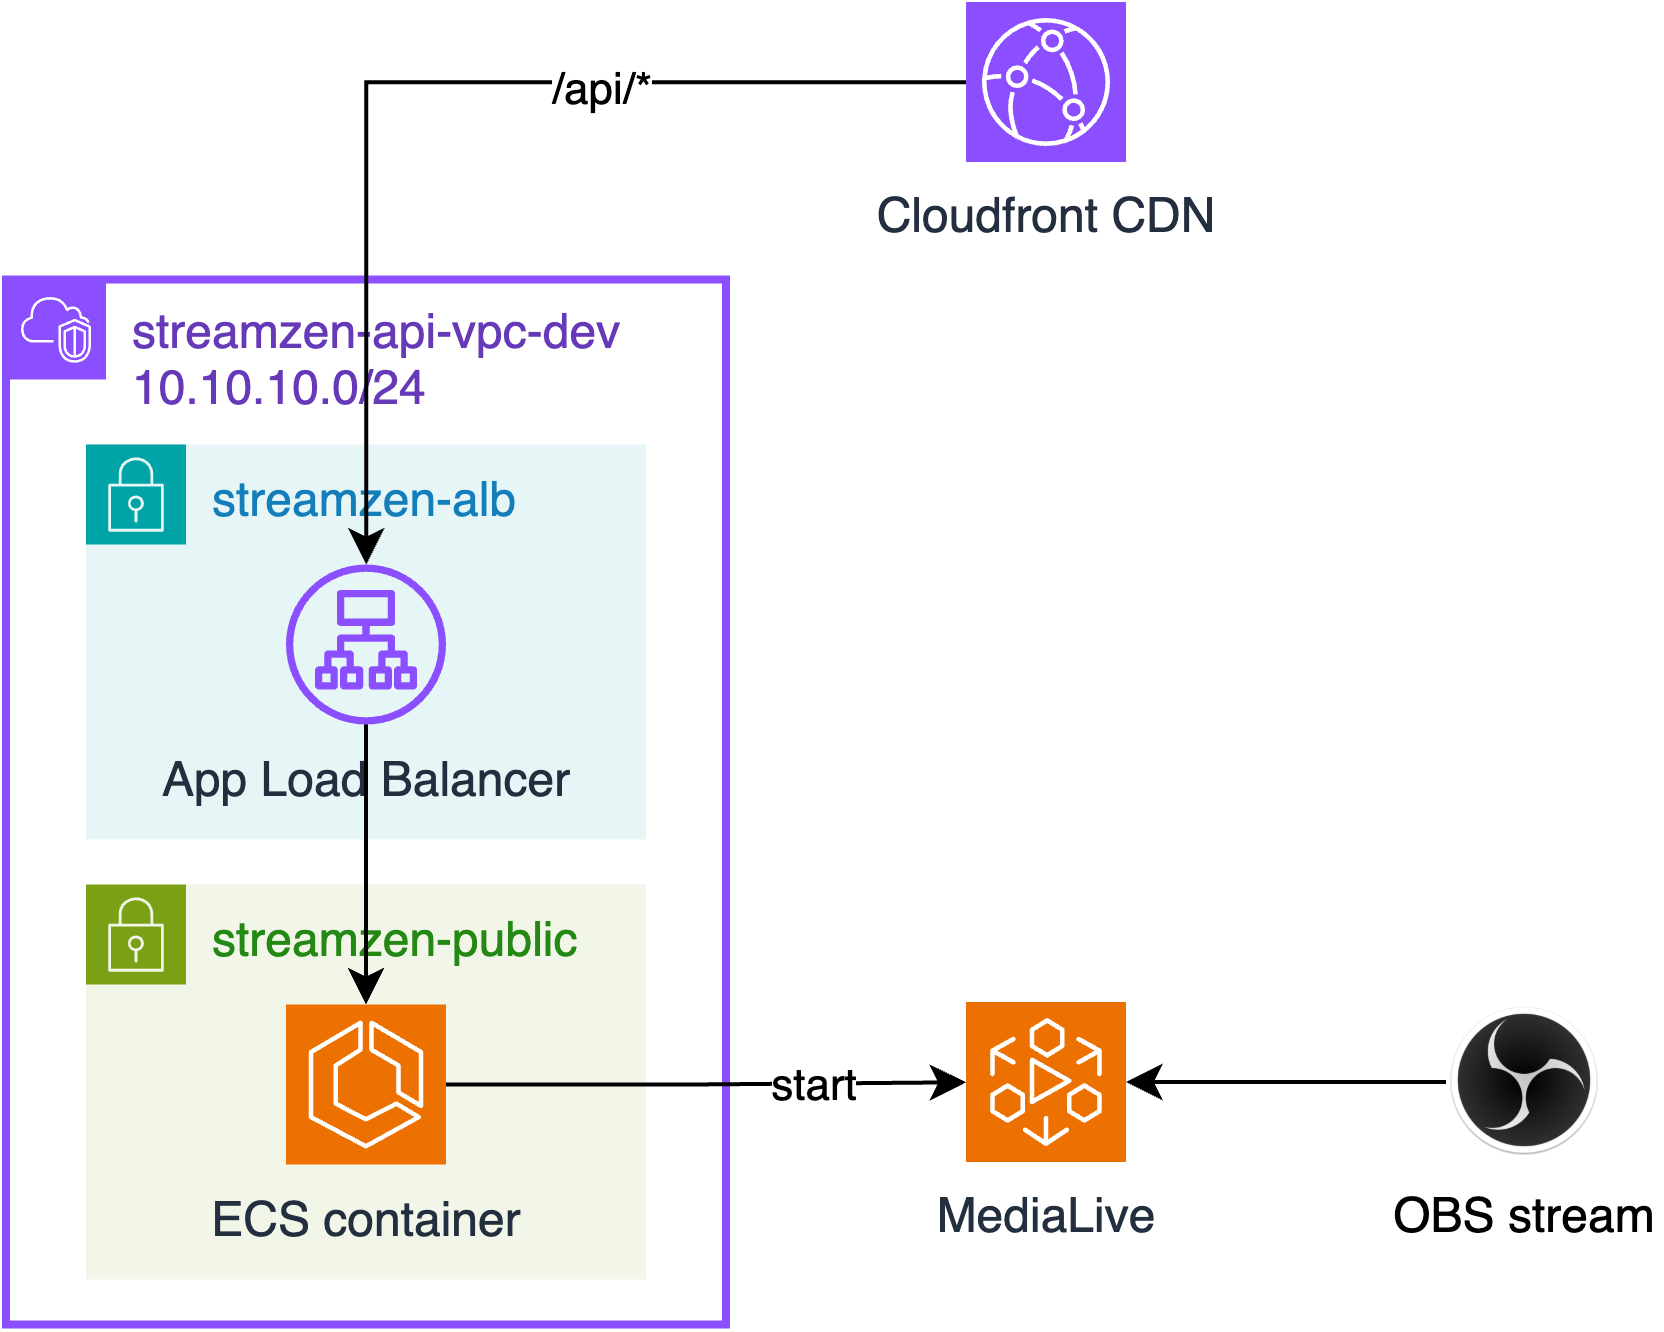
\includegraphics[width=120mm, keepaspectratio]{figures/dipterv_live1.png}
	\caption{Folyamatábra a live stream indításáról.}
	\label{fig:live1}
\end{figure}

\begin{figure}[ht]
	\centering
	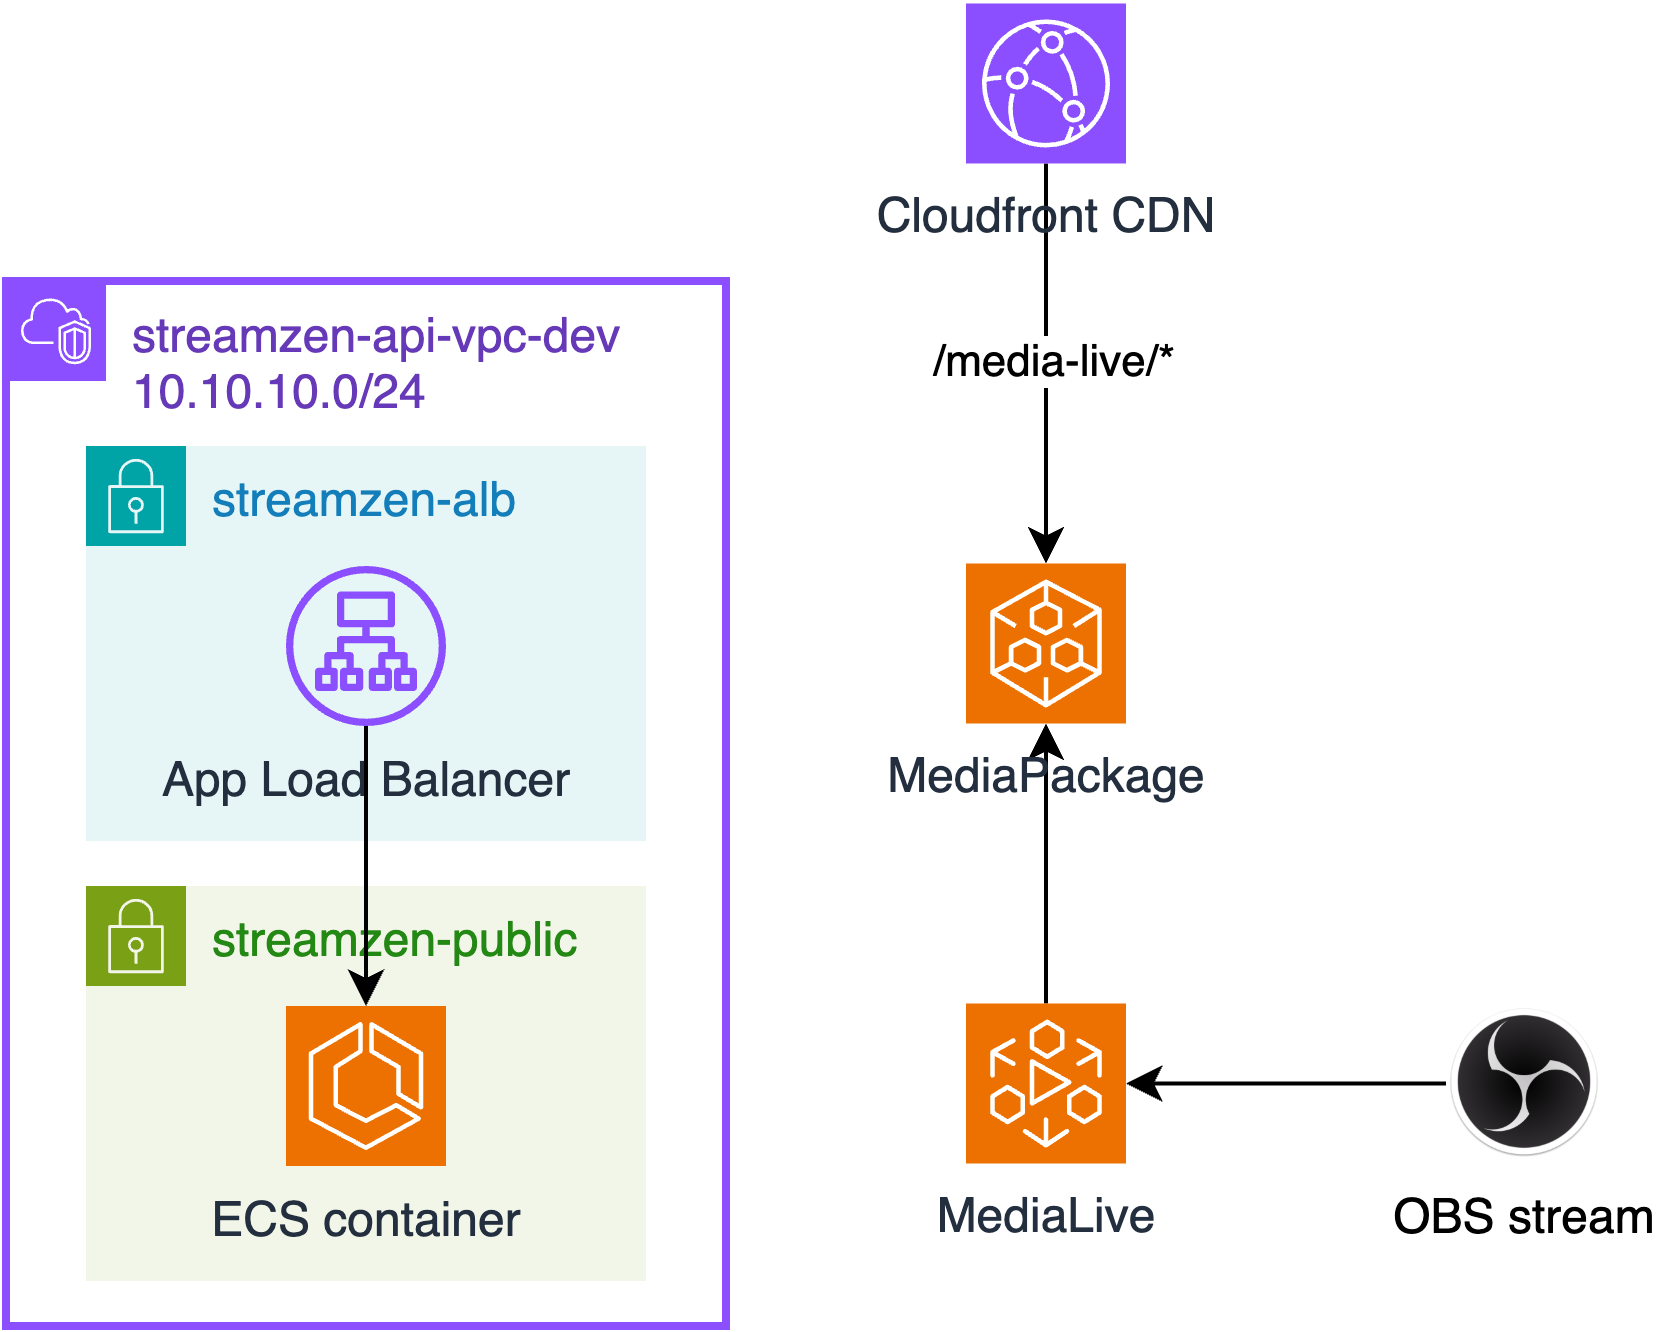
\includegraphics[width=120mm, keepaspectratio]{figures/dipterv_live2.png}
	\caption{Folyamatábra a live streamre való kapcsolódásról.}
	\label{fig:live2}
\end{figure}

\section{Konfigurációmenedzsment}

TODO: Terraform választásának indoklása. Kialakított Terragrunt module rendszer. GitHub actions a Terraform tervek előnézetére, OIDC felállítása az AWS role felvételére.
